\section{Problem 2}

In this problem we analyse the Vandermonde matrix and use various techniques to solve it. The way I formatted this is by first listing the whole code, and then per sub-question discussing the output of relevant part of the code. I did this because some of the code overlaps between sub-questions. Per sub-question, I indicate in the code the part relevant to it (e.g. \#2A). The very beginning is copied from the recommended routine of the Exercise set, as well as some plots. The code I have written is as follows: 

\lstinputlisting{NURhandin1_2.py}

\newpage
\subsection{Problem 2a}

First we take a look at problem 2a. In this problem, the goal is to write a code that does an LU decomposition of the Vandermonde matrix and use the resulting LU matrix to obtain the solutions $c_i$ for data points $x_i$, where i = 0,1,...,19. First of all, we create the matrix V. We do this by taking every row to be (1, $x_i$, $x_{i}^2$, ...., $x_{i}^{19}$), again for our different 20 data values $x_i$, filling j = 1,2,...,19 rows in total. In order to first obtain the LU matrix, we apply the $\textbf{improved Crout's algorithm}$ from lecture 3 slide 15 as shown in the code. As can be seen in the code, we first take our LU matrix as the input matrix V (as instructed on slide 13), and gradually swap and overwrite different elements of the matrix. If an input matrix is not square, we return an error message that no LU matrix can be found for a singular matrix. All used for loops can be translated to summing for different values i within the range of the loop. The if-statements determine the conditions for which we should apply operations. After we finish all loops, we return a matrix LU of equivalent shape to V that contains our $\alpha_{ij}$ and $\beta_{ij}$ values, which we will require to apply forward- and backward substitution.\\

Next, using the LU matrix and the given $\vec{b}$=$y_i$ data values, we apply a $\textbf{forward subtitution algorithm}$ inspired by slide 11 of lecture 3. The diving by $\alpha_{ii}$ factors are omitted because we have set these values to be equal to 1 implicitly. From this rather straightforward algorithm, we (confusingly) obtain the y values we require to apply $\textbf{backward subtitution}$. This algorithm is a bit more complicated. We go through this loop in reverse order, applying numerous operations to construct our solution vector x. These operations include dividing by $\beta_{ii}$ and multiplying by $\beta_{ij}$ and $y_i$ values respectively for j $>$ i, opposite from the conditions from the forward subtitution, j $<$ i. Finally, we combine these three seperate algorithms into a final function in which we can input the matrix we want to solve A and it's solution $\vec{b}$. In our case, we will use V and $\vec{y}$ respectively for this. This function then returns a vector of x-values. These are the c-values we wished to obtain, given by:

\lstinputlisting{problem2a.txt}

Using these c values, we can calculate (interpolate) the y values by applying equation (2) from the hand-in set with the 1000 x values we want to interpolate at. Next, we plot the resulting 1000 y values together with the 20 y points from the data to see how they match:

\begin{figure}[h!]
  \centering
  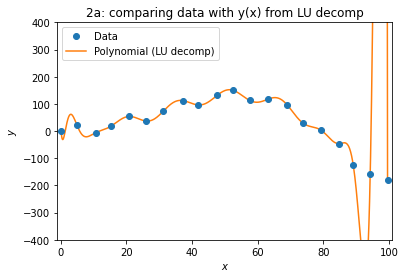
\includegraphics[width=0.6\linewidth]{problem2a1.png}
  \caption{The polynomial y(x) obtained with the LU decomposition method plotted together with the given data points to test whether it intersects them.}
  \label{fig:fig1}
\end{figure}

From this figure we can conclude that we get a pretty good description of the data, except for x values below 5 and especially above 90. At x values close to the maximum, the polymial seems to vary wildy. Despite this, it still does go through the data points somewhat well as seen in the plot. The accuracy does decrease at these higher x values though, as can be seen in the second plot below, where we calculate the absolute value of the error per data point. I use a logarithmic scale to see the error values more clearly:

\begin{figure}[h!]
  \centering
  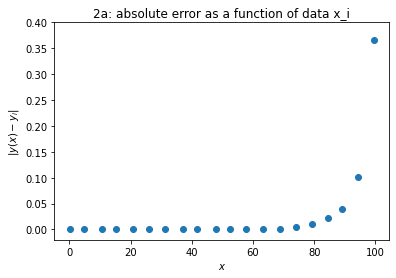
\includegraphics[width=0.6\linewidth]{problem2a2.png}
  \caption{The absolute difference between the polynomial y(x) and the data points $y_i$ to visualise how far off the polynomial is from the actual data. This y-scale seemed most appropiate as you can spot differences between individual points. Smaller x values seem to have exponentially smaller error values.}
  \label{fig:fig2}
\end{figure}

All in all, the result is quite satisfactory, as both visually and quantitatively, the polynomial seems to describe the data points fairly well, save for the aforementioned boundary cases. 

\subsection{Problem 2b}

For this next sub-question, we are supposed to implement $\textbf{Neville's algorithm}$ to find interpolated y values for a given input array of x values between 0 and 20. To apply this algorithm, we first write a $\textbf{bisection algorithm}$ to find the index $j_{low}$, which is the closest index to the index of our x value we want to interpolate at. In our bisection algorithm, we first treat the cases were there is extrapolation, meaning the x value falls outside of the range of xdata values. In this case, we simply take the indices around the edges to interpolate with like in problem 1 of tutorial 2. Next, we set up a start, end and size index. An important note is the way the algorithm is written, the start index will be equivalent to the $j_{low}$ index and will be updated as we continue. From these we can implicitly construct a left and right half range of indices of the sample values. After this, we go into a while loop and update our left and right index ranges as we continue to narrow down the ranges. We quit this process once we find that the difference in start and end indices falls below 1, because that means the indices start to overlap, which is something we want to avoid as at this point we already found the closest indices. After we reach this threshold, we take the start value, which is the lower closest index (the value is floored), and compare this for a set of cases. If this index (remember this is $j_{low}$) is either smaller than the given order or the index plus the order exceed the amount of data points, we return 0 and $j_{low} - \text{order}$ respectively. For the non-edge cases however, we obtain the smallest index $j_{low}$.\\

Moving on to Neville's algorithm, from $j_{low}$ we find the total range of M tabulated points around x given by $[j_{low},j_{low}+M-1]$. As we have a 19th degree polynomial in this case, we use an input value of M = 20, as this is equivalent to order (M-1 =) 19. We copy both the y and x values of the data in P and xdata respectively in the range of $[j_{low},j_{low}+M-1]$. Next we create a nested for loop in which we loop k from 1 to M-1 and i from 0 to M-1-k. In this loop we fill P with y values and compute the Lagrange polynomial using subsequent indices. We do this until we break out of the loop over i, which leaves us with the interpolated value as the 0th element of the P array. To get our 1000 interpolated y values we apply this algorithm to each of the 1000 points seperately and also for the 20 values matching the data in order to make another error comparison plot. The resulting comparison between the Lagrange polynomial found using this algorithm and the data is plotted below:

\begin{figure}[h!]
  \centering
  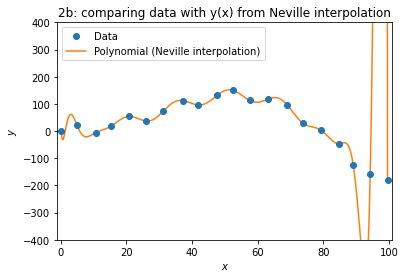
\includegraphics[width=0.6\linewidth]{problem2b1.png}
  \caption{The polynomial y(x) obtained from 1000 x values from 0 to 20 interpolated using Neville's algorithm. This Lagrange polynomial is plotted together with the given data points to test whether it intersects them.}
  \label{fig:fig3}
\end{figure}

Visually, the polynomial seems very similar to the one found in the first problem. We can verify this by plotting together the absolute error per data point for both the polynomial found using LU decomposition and Neville's algorithm, again using a logaritmic scale: 

\begin{figure}[h!]
  \centering
  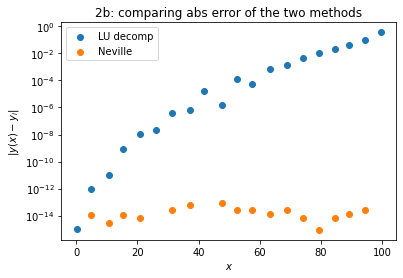
\includegraphics[width=0.6\linewidth]{problem2b2.png}
  \caption{The absolute difference between the polynomial y(x) and the data points $y_i$ to visualise how far off the polynomial is from the actual data. This y-scale seemed most appropiate as you can spot differences between individual points. Smaller x values seem to have exponentially smaller error values.}
  \label{fig:fig4}
\end{figure}

\subsection{Problem 2c}

In this problem we want to try and improve our result by performing multiple iterations of LU decomposition. There are namely unknown errors $\delta x$ present in our found solution, or in this case, errors $\delta c$ of the solutions $c_i$. Before I tackle the problem, we will be needing matrix multiplication. For this I write a very simple function $\textbf{matrix multiplication}$ that takes an input square matrix A and vector $\vec{x}$ and outputs their matrix product with dimensions equal to $\vec{x}$. Using lecture 3 slide 18 as a guideline, we explain it as follows, following along in the code in the function $\textbf{LU iterations}$:\\
In problem 2a, we have found a solution of the form V$\vec{c}$ = $\vec{y}$. There is some unknown error on this however: $\vec{c'}$ = $\vec{c}$ + $\vec{\delta c}$. We can then rewrite to V$\vec{c'}$ = V($\vec{c}$ + $\vec{\delta c}$) = $\vec{y}$ + $\vec{\delta y}$, where we save the right-hand side of this equation as $\delta b$. To obtain the aforementioned error value, we can then do another LU decomposition with this $\delta b$ to obtain a solution for the error values. We then obtain a new solution $\vec{c''}$ = $\vec{c'}$ - $\vec{\delta c}$ found by, as the function shows, subtracting the found error from our initial, 'lower order' solution. We append the function to iterate this 10 times, leaving us with a 10th order solution for $c_i$, given by $\vec{c}^{(10)}$. As we have done before, we then fill both an array with 1000 and 20 interpolated values to compare with the data points and 1 LU iterations respectively. For the data comparison, the plot is as follows:\\

\begin{figure}[h!]
  \centering
  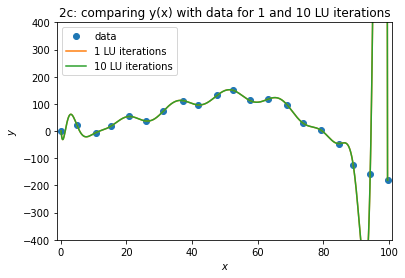
\includegraphics[width=0.5\linewidth]{problem2c1.png}
  \caption{The polynomial y(x) obtained from 1000 x values from 0 to 20 interpolated using both 1 and 10 LU iterations. This Lagrange polynomial is plotted together with the given data points to test whether it intersects them. We see no clear difference between 1 and 10 LU iterations; the polynomials overlap.}
  \label{fig:fig5}
\end{figure}

Next, we plot the comparison in absolute error between the Lagrange polynomial and the data for both 1 LU and 10 LU iterations. The result is:\\

\begin{figure}[h!]
  \centering
  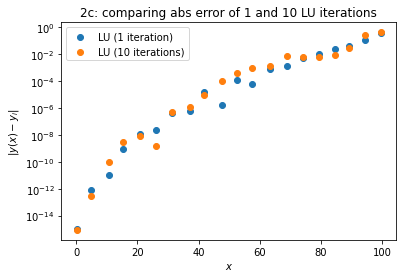
\includegraphics[width=0.5\linewidth]{problem2c2.png}
  \caption{The absolute error compared for 1 and 10 LU iterations. We see that while small, the error actually seems to increase for more LU iterations.}
  \label{fig:fig6}
\end{figure}

\subsection{Problem 2d}

In this final problem we time the execution times of problems a), b), and c). We do this by importing the $\textit{timeit}$ module and defining a variable per sub-question that starts a timer. We then loop through the entire code of the sub-question $k$ number of times. To then find the average execution time, we define another variable in which we print out the difference between the current time minus the starting time, divided by the number of executions $k$. Doing this for an adequate number of execution times (a: k=50, b: k=10, c: k=20) to give a consistent result, we find that the code from a), so doing LU decomposition, is by far the fastest method to find the Lagrange polynomial. Followed up by this is the code from problem c) in which we perform 10 LU iterations, which appears to be some margain slower than just 1 LU decomposition, which you'd expect as you are iterating the code from a) multiple times essentially. Finally, we see that the code in b) is by far the slowest method to find the Lagrange polynomial. Especially when compared to just LU iteration, it takes significantly longer to execute. Relatively, we find that $\frac{t_b}{t_a} \approx 18$, $\frac{t_b}{t_c} \approx 3$ and $\frac{t_c}{t_a} \approx 6$.\\

Therefore, the LU decomposition method to find y(x) from problem 2a) appears to be the most efficient. It takes the least amount of time by a large margain and finds a relatively accurate description of the data. Subsequently, we conclude that Neville's algorithm from problem 2b) is the least efficient method as it takes significantly longer to find. The method from problem 2c), multiple LU iterations, is still more efficient than Neville's algorithm if you keep under a certain number of iterations. Testing around, Neville's algorithm seems to be faster if you exceed about 35 LU iterations.\\

In terms of accuracy we can tell by figure 4, the plot of absolute error of Neville compared to the LU decomposition, that Neville's algorithm seems to give more accurate results per data point. This confirms the logical conclusion one would tend toward when seeing the execution times: it seems that using Neville's method is less efficient in terms of operations but provides the most accurate result, while using LU decomposition is the opposite in that it's less accurate but much more efficient. So to conclude I expect Neville's algorithm to be the most accurate method to construct the Lagrange polynomial, but if you value efficiency more it is likely best to use LU decomposition instead, as the differences between the two seem very small. The output of the run times are:\\

\lstinputlisting{problem2d.txt}